%#Split: 02_purpose_plan  
%#PieceName: p02_purpose_plan
% p02_purpose_plan_00.tex
\KLBeginSubjectWithHeaderCommands{02}{}{研究目的・内容等}{2}{F}{}{\DCPDFirstSubjectPageStyle}{\DCPDDefaultPageStyle}

\section{研究目的・内容等}
%    <<最大 2ページ>>

%s02_purpose_plan_dcpd
%begin 研究目的と研究計画short留意事項なし ====================
%begin 研究計画における研究目的、研究方法、研究内容 ====================
\graysubsection{①研究計画における研究目的、研究方法、研究内容}
\vspace{20pt}
\sbsbsection{研究目的}
本研究では、利用者に直接反応を伺うシステムを構築することで、新たなフェイクニュース早期検出の枠組みを作る。
またフェイクニュースの早期自動検出を日本語で実現・研究の促進を目指し、
データセットの作成から検出モデルの実装を目的とする。

\sbsbsection{研究方法・研究内容}

\setlength\intextsep{0pt}
\setlength\textfloatsep{0pt}
\begin{wrapfigure}{r}[0pt]{0.29\linewidth}
    \vspace{-2\baselineskip}
    \centering
    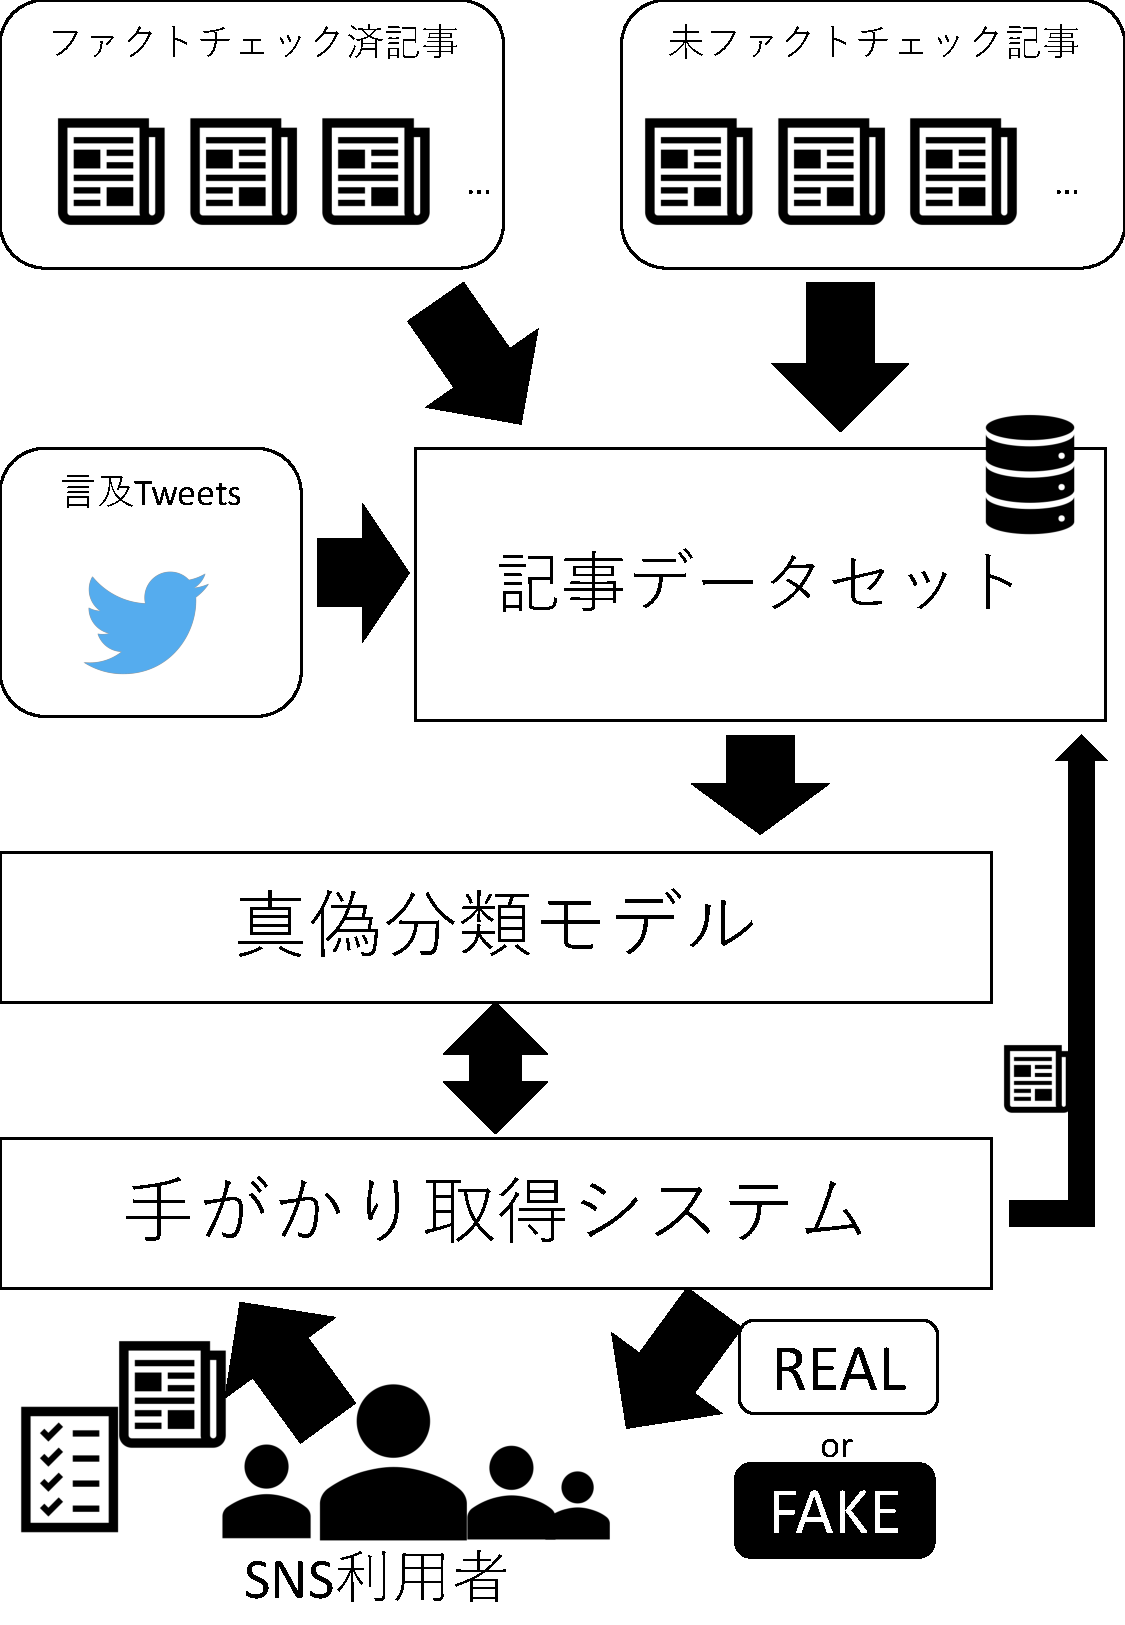
\includegraphics[width=0.29\textwidth]{figs/final.pdf}
    \vspace{-1cm} 
    \caption{本研究計画の完成予想図。}
    \label{fig:dataset}
    \vspace{-3\baselineskip}
\end{wrapfigure}

以下の3目標を目指し研究する。
\begin{description}
    \item[目標Ⅰ] 新たな検出コンセプトとしてSNS上で利用者へ反応を促すことでさらなる早期検出を実現するシステムの構築を目指す。
    \item[目標Ⅱ] 日本語データセット作成に向けファクトチェック済記事とそうでない記事、同時にSNS上で記事に寄せられたコメントや利用者情報等を収集する。
    \item[目標Ⅲ] 早期検出を想定した状況で高精度な真偽分類を行うモデルを利用者の初期反応から得られた情報と共に行う。
    %\item[目標Ⅲ] 利用者に対して直接フェイクニュースの疑いを指摘すると同時にデータセットのアップデートを行うモデルを開発する。
\end{description}

%end 研究計画における研究目的、研究方法、研究内容 ====================

%begin どのような計画で、何を、どこまで明らかにしようとするのか ====================
\graysubsection{②どのような計画で、何を、どこまで明らかにしようとするのか}
\vspace{20pt}
\sbsbsection{目標Ⅰ: SNS上で利用者へ反応を促すことでさらなる早期検出を実現するシステムの構築(採用前 - 1年目)}
データセットとモデルの構築のみでは、今後のニュース内容の変化に対応することが難しい。
継続して社会の潮流の変化に対応するためには、データセットと検出方法及び利用者の反応を得る方法を工夫する必要がある。
%また、本研究の最終的な目標は国連のPause/ちょっと待って運動\cite{un}と同じくSNS利用者に対してフェイクニュース拡散前に利用者に再考を促して抑止を行うことである。
%この実現には、検出モデルの構築のみならず\underline{利用者に対し納得できる形で記事の疑わしさを提供するシステムの構築}により初めて実現する。
本研究では、SNS上で利用者に対して反応を促すことで早期検出の性能向上に繋げる新しいモデルを実装する。
実現形式として、
フェイクの疑いが強いと判断された記事に対してキュレーターの役割であるリプライを飛ばしたり、
利用者が信憑性を問い合わせたい記事に対し簡易的なチェックリスト(文体が感情的か・著者は明記されているか等)を課して回答を得たりする方法などを検討している。
%本研究は、利用者がモデルに直接真偽を問い合わせるシステムを構築する。
%上記で実装したモデルに対して、利用者が記事内容を入力し問い合わせることで、
%真偽判断結果を提供すると共にデータセットへラベルなしニュースの追加を狙う。
実験ではSNS利用者を対象とした主観評価実験により、\underline{フェイクニュース拡散の抑止効果}を測定するほか、。
モデル提供が難しい場合は、データセットを公開し日本語におけるフェイクニュース早期検出研究促進を目指す。
%技術的チャレンジングさも書く
%利用者が疑わしい記事なのか早く知りたい→ファクトチェック結果を
%踏みとどまれの根拠をもたせる→国連


\sbsbsection{目標Ⅱ: 日本語の記事・真偽を含むデータセットを作成する(1年目 - 2年目)}
\setlength\intextsep{0pt}
\setlength\textfloatsep{0pt}
\begin{wrapfigure}{r}[0pt]{0.7\linewidth}
    %\vspace{-2\baselineskip}
    \centering
    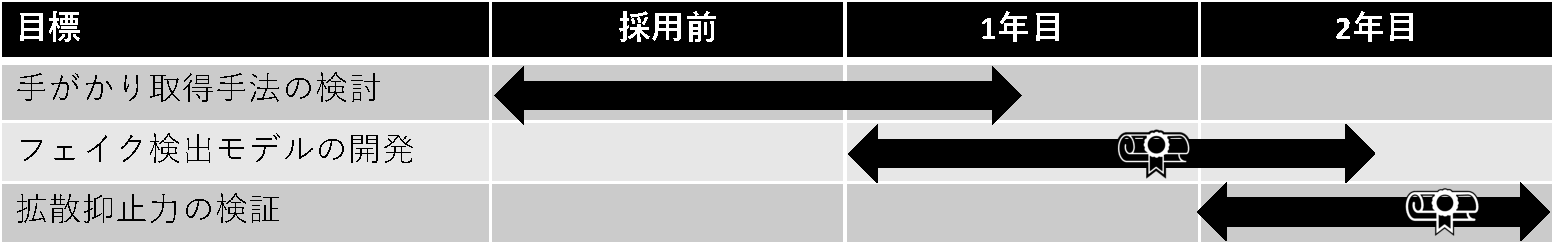
\includegraphics[width=0.7\textwidth]{figs/plan.pdf}
    \vspace{-1cm} 
    \caption{研究計画の年毎の流れ。}
    \label{fig:plan}
    %\vspace{-3\baselineskip}
\end{wrapfigure}
日本語での検出を実現するためには、まずはデータセットを作成する必要がある。
データセット作成の全体の流れは図\ref{fig:dataset}の通りである。
%完全教師あり学習・弱教師あり学習に問わず最低限必要なものは記事情報とファクトチェック結果による真偽ラベルである。
日本語ファクトチェック結果の取得には、特定非営利活動法人ファクトチェック・イニシアティブ(以下FIJ)が提供するFactCheck Naviを使用する。
2021年4月現在で600超件のファクトチェック結果が公表されている。%おり、FIJが提供するガイドライン\cite{fij}に基づき9種類のレーティングが行われている。
%今回はその中で``誤り''、``虚偽''、``ミスリード''、``不正確''、``根拠不明''と評価された記事をフェイクと扱う。
一方ファクトチェックにより正確と判断された事例はフェイクに比べて少な%く、2021年4月中旬現在FactCheck Naviの直近20件のファクトチェック結果は全てフェイクに該当する。
いため、正確なニュースとして大手新聞社やロイター通信等の記事を収集する。

また目標Ⅲに向けファクトチェックが行われておらず、正解ラベルがない記事も追加する。
正確とみられるニュースは先述と同じく大手マスメディアが発信したニュースを扱い、
疑わしい記事としてFactCheck Naviによって虚偽と複数回判断されたニュースサイトの他記事も収集対象とする。
最終的には真偽合わせて\underline{ラベル付き記事を約1,200件}、\underline{ラベルなし記事を約5,000件以上}収集を目指す。
利用者の反応として、全記事を対象にSNS上で寄せられたコメントとしてTwitterにて記事URLを含むツイートも収集する。

\sbsbsection{目標Ⅲ: 弱教師あり学習によってラベル不足を補うモデルを構築する(2年目)}

ラベル付き利用者の反応を弱いアノテーションとして扱ってフェイクニュースを検出する方法は、
英文記事を対象にしたKai Shuらの研究で1例が示されている\cite{shu2020leveraging}。
ここではコメント群の感情値の標準偏差やコメント者の過去の投稿、そしてフォロー関係から弱いアノテーションを付加している。
これら3種の弱いアノテーションも併せて学習することで、推論時は利用者の反応を使わずに正確な早期検出を実現した。
日本語で実現を目指す場合、日本語での検出を行う研究が少なく言語の違いによる影響が未知数であるため\underline{大幅なモデルの改変を要する可能性}がある。
今回は日本語での早期検出実現に向けて3種類の弱いアノテーションに加え、投稿者のプロフィールや使用された絵文字、ハッシュタグといったコメント情報で有用なものがないか模索する。
実験では、\underline{学習時には記事と利用者の反応を入力に扱い、テスト時は記事のみを入力}して早期検出時の状況を再現し既知の手法と比較する。
既知の手法と比較して検出性能の改善がみられた場合は成功とみなす。
%技術的チャレンジングさを強く主張する
%高速化させたい→そのために???を克服しなければならない
%学術的チャレンジングさ→日本語がない→言語的差異+研究がないので英語の流用でいいのか未知数

%end どのような計画で、何を、どこまで明らかにしようとするのか ====================

%begin 研究の特色・独創的な点 ====================
\graysubsection{③研究の特色・独創的な点}
\vspace{20pt}
\sbsbsection{本研究の特色}
\begin{itemize}
    \setlength{\parskip}{0cm}
    \setlength{\itemsep}{0cm}
    \item 能動的に\underline{利用者から情報提供を得た上}で、\underline{継続してデータセット拡大・モデル改善}を行う点。
    \item \underline{日本語}を対象にフェイクニュースの自動検出を行う点。
    \item ファクトチェックの結果を待たず\underline{早期の検出}を目指す点。
\end{itemize}
\vspace{-10pt}
\sbsbsection{独創的な点: 先行研究との比較}
先行研究は利用者の反応を利用する場合該当情報を時間が経過してから取得する受動的な形を取り、
形式もSNSプラットフォーム(Twitter, Instagram, etc.)によって微妙な差異がみられる。
本研究では\underline{能動的に利用者の反応を得る}枠組みを作り、今後\underline{主流SNSが変化しても早期検出の実現}が可能となる。

また深層学習でフェイクニュースを自動検出する\underline{研究対象は英文に集中}し、
\underline{日本語データセットがない}。
言語に囚われず利用者による拡散された経緯で真偽を判断する研究もあるが\cite{tarek2020}、
依然として記事の内容を考慮した研究では日本語を対象としたものがない。

\sbsbsection{独創的な点: 予想されるインパクト・将来の見通し}
総務省によるとSNS利用率は2019年現在69\%を占める上、SNSマーケティング市場規模は2025年に1兆1,171億円まで成長する(出典:サイバー・バズ/デジタルインファクト調べ)と推測されている。
% インシデントを重ねて書く
SNS利用者の増加によって、今後フェイクニュースは\underline{更に深刻な社会損害}を起こし、\underline{謂れなき風評被害に悩む事例の増加}が想定される。
本研究の完成によりこれまで活発になされていなかった日本語のフェイクニュースを早期検出するモデルの開発および提供が可能となる。
SNS利用者への注意喚起に活用ができるほか、ファクトチェックを行う人への補助システムへの活用
といった様々な形式でSNS上で騙される人を減らし\underline{社会的損害や風評被害を未然に防ぐ}枠組み作りに貢献する可能性がある。

%end 研究の特色・独創的な点 ====================

%begin 申請者が担当する部分 ====================
\graysubsection{④申請者が担当する部分}
本研究は所属研究室内でも萌芽的な取り組みで、環境・技術面の支援を除き\underline{申請者が全部分を担当}する。
データセットの生成では、正確なニュースの取得へ大手マスメディアへ協力を求める可能性がある。
%end 申請者が担当する部分 ====================

%begin 受入研究機関と異なる研究機関での研究従事計画 ====================
\graysubsection{⑤受入研究機関と異なる研究機関での研究従事計画}
私は\underline{1年間タリン工科大学の言語技術研究所(Tanel Alumäe所長)で活動予定}である。
当該分野は北米と欧州の研究が活発であることから、\underline{最前線の研究に従事}するために必要である。
%end 受入研究機関と異なる研究機関での研究従事計画 ====================

%\vspace{1cm}
{\footnotesize 
\begin{twobibliography}{99}
    \setlength{\parskip}{0cm}
    \setlength{\itemsep}{0cm}
    %\bibitem{fij} FIJ. 2019: ファクトチェック・ガイドライン
    \bibitem[9]{shu2020leveraging} K. Shu, \textit{et al.} \textit{ECML-PKDD 2020}
    \bibitem[10]{un} UNIC. \url{https://is.gd/UNIC_pause}. 2020
    \bibitem[11]{tarek2020} T. Hamdi, \textit{et al.} \textit{ICDCIT 2020}
\end{twobibliography}
}
%end 研究目的と研究計画short留意事項なし ====================
% p02_purpose_plan_01.tex
\KLEndSubject{F}


